\documentclass[11pt]{article}

\usepackage{pablo}
\usepackage{pgfplots}
\usepackage{ifthen}
\usepackage[a5paper,margin=1.8cm]{geometry}

\pagestyle{empty}
\begin{document}

\begin{center}
  {\large
    DM
    ---
    \textsc{Statistiques --- Raisonnement}
  }
\end{center}

\emph{À rendre le vendredi 22 novembre}

\begin{exercice}
  Alain, intéressé par la météorologie, mesure les précipitations chez lui
  toutes les semaines. Il part quinze jours en vacances pendant les semaines 6
  et 7, et n'a donc pu faire qu'un relevé pour ces deux semaines.

  \hspace{-2.5em}\begin{tabular}{l|cccccccc}
    Semaine & 1 & 2 & 3 & 4 & 5 & 6 et 7 & 8 & 9 \\
    \hline
    Précipitations (mm) & 15 & 14 & 14 & 16 & 17 & 31 & 16 & 17 \\
  \end{tabular}

  Afin de visualiser les précipitations, il trace l'histogramme suivant.

  \begin{center}
    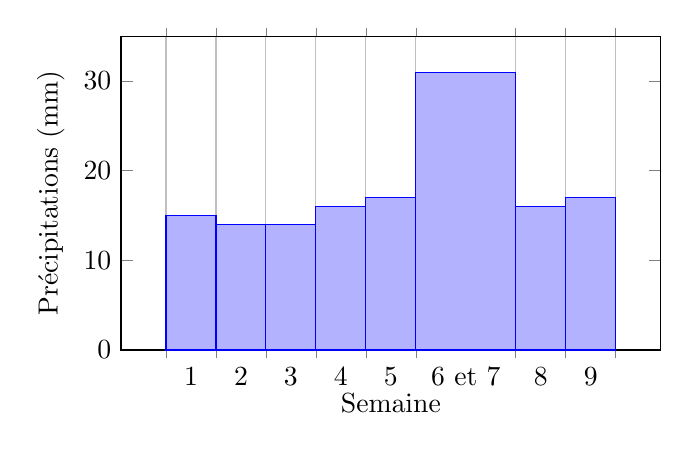
\begin{tikzpicture}
      \begin{axis}[
          yscale=0.7,
          ymin=0,
          ymax=35,
          xlabel=Semaine,
          ylabel=Précipitations (mm),
          ybar interval,
          xtick=data,
          xticklabel={\ifthenelse{\equal{\tick}{6.0000000000}}{6 et 7}{\pgfmathprintnumber\tick}},
        ]
        \addplot coordinates {
          (1, 15)
          (2, 14)
          (3, 14)
          (4, 16)
          (5, 17)
          (6, 31)
          (8, 16)
          (9, 17)
          (10,17)
        };
      \end{axis}
    \end{tikzpicture}
  \end{center}
  \begin{enumerate}[(1)]
    \item Selon son histogramme, quelles semaines ont eu lieu les plus fortes précipitations ? Cela reflète-t-il la réalité ?
  \end{enumerate}
  L'erreur d'Alain est qu'il a fait \emph{les hauteurs} des barres proportionnelles à
  la valeur des caractères, alors que \emph{les aires} des barres auraient dû être
  proportionnelles à la valeur des caractères.

  Le but de cet exercice est de tracer un histogramme correct.

  \begin{enumerate}[(1)]
      \setcounter{enumi}{1}
    \item Dans cette question nous allons compléter le tableau de
      proportionnalité suivant, où les trois dernières lignes correspondent aux
      barres de l'histogramme que nous tracerons ensuite.

      \hspace{-1.5em}\begin{tabular}{p{7em}||c|c|c|c|c|c|c|c}
          Semaine & 1 & 2 & 3 & 4 & 5 & 6 et 7 & 8 & 9 \\
          \hline
          \hline
          Précipitations (mm) & 15 & 14 & 14 & 16 & 17 & 31 & 16 & 17 \\
          \hline
          \hline
          Aire &   & 7 & & & & &\\
          \hline
          Largeur & 1 & 1& 1& 1& 1& 2& 1& 1\\
          \hline
          Hauteur &&&&&&&
        \end{tabular}

      \begin{enumerate}[(a)]
        \item Remplir la ligne « Aire », de sorte que l'aire soit
          proportionnelle aux précipitations.
        \item Remplir la ligne « Hauteur », de sorte que dans chaque colonne, le produit de la hauteur par la largeur soit égale à l'aire.
      \end{enumerate}
    \item Tracer l'histogramme en utilisant les largeurs et hauteurs des barres calculées dans le tableau.
  \end{enumerate}
\end{exercice}

\begin{exercice}[Établir une égalité]
  Voici trois méthodes pour établir une égalité.
  \paragraph{Méthode 1} On transforme par étape successive un membre de l'égalité à établir pour obtenir le second.

  \begin{em}
    Exemple : Montrer que $(x-2)(x+3)=x^2+x-6$.

    On part du premier membre : 
    \begin{eqnarray*}
      (x-2)(x+3) &=& x\times x + 3x-2x-2\times 3\\
                 &=& x^2 + (3-2)x -6\\
                 &=& x^2 + x - 6
    \end{eqnarray*}
    Puisqu'on retrouve le second membre, l'égalité est vraie.
  \end{em}

  \paragraph{Méthode 2} On transforme chaque membre de l'égalité pour montrer qu'ils sont égaux à une même quantité.

  \begin{em}
    Exemple : Montrer que pour tout réel $x$, $x(x+1)(x+2)(x+3)=(x^2+3x+1)^2-1$

    On développe le premier membre :
    \begin{eqnarray*}
      x(x+1)(x+2)(x+3) &=& x(x+1)(x^2+5x+6)\\
                       &=& x(x^3+6x^2+11x+6)\\
                       &=& x^4+6x^3+11x^2+6x
    \end{eqnarray*}

    On fait de même pour le second membre :
    \begin{eqnarray*}
      (x^2+3x+1)^2-1 &=& (x^4+3x^3+x^2)+\\
                     & & (3x^3+9x^2+3x)+\\
                     & & (x^2+3x+1)-1\\
                     &=& x^4+6x^3+11x^2+6x
    \end{eqnarray*}

    On trouve donc : $x(x+1)(x+2)(x+3)=x^4+6x^3+11x^2+6x=(x^2+3x+1)^2-1$. Les deux quantités sont donc égales.
  \end{em}

  \paragraph{Méthode 3} On calcule la différence des deux membres, et on montre qu'elle est nulle.

  \begin{em}
    Exemple : Montrer que $\dfrac{1}{\sqrt 2}=\dfrac{\sqrt 2}{2}$.

    \begin{eqnarray*}
      \frac{1}{\sqrt 2}-\frac{\sqrt 2}{2} &=& \frac{1}{\sqrt 2}\times\frac{2}{2} - \frac{\sqrt 2}{2}\times\frac{\sqrt 2}{\sqrt 2}\\
                                          &=& \frac{2}{2\sqrt 2}-\frac{\sqrt 2\times\sqrt 2}{2\sqrt2}\\
                                          &=& \frac{2}{2\sqrt 2}-\frac{2}{2\sqrt 2}\\
                                          &=& 0
    \end{eqnarray*}
  \end{em}

  En précisant le numéro de la méthode utilisée, démontrer que :
  \begin{enumerate}[(a)]
    \item Pour tout nombre réel $a$, $a^3-1=(a-1)(a^2+a+1)$.
    \item Pour tout nombre réel $x$, $(x-3)(x^2+3x-10)=(x+5)(x^2-5x+6)$.
    \item Pour tous points du plan $A$, $B$, $C$, $D$ :\\ $\vecteur{AB}+\vecteur{CD}=\vecteur{AD}+\vecteur{CB}$.
    \item $\dfrac{\sqrt5-\sqrt2}{\sqrt3}=\dfrac{\sqrt3}{\sqrt5+\sqrt2}$.
    \item Pour tout nombre réel $x$ différent de 1:\\ $\dfrac{2x^2-5x-1}{x-1}=2x-3-\dfrac{4}{x-1}$.
  \end{enumerate}
\end{exercice}

\end{document}
